\chapter{Literature Survey}\label{ch:2}
\section{LightWeight Adaptive Binary Translation}
\label{adaptive_binary_translation}
The virtualization overheads of trap-and-emulate style virtualization can be up to 20x for compute-intensive workloads executing a large number of privileged instructions (Table~\ref{tab:kvm_performance}). The primary source of overhead are VM-exits due to guest privileged instructions. Table~\ref{tab:priv_opcodes} lists the most executed privileged opcodes and briefly explains their semantics. Figure~\ref{fig:opcode_exit_fraction} shows the percentage of exits caused due to each opcode. Only five opcodes result in more than 80\% of exits on all three benchmarks. Table~\ref{tab:exitcount_linuxboot} presents the frequency profile of VM exits on the Linux boot benchmark in more detail.

In adaptive binary translation, number of distinct program counter (PC) values that cause exits are profiled and are translated to corresponding non privileged VMM logic. Figure~\ref{fig:pc_profile} shows a histogram on the number of distinct PC values and the frequency of exits on them. Table~\ref{tab:pcexits_linuxboot} presents the exit profile of different PCs in more detail for the Linux boot benchmark. For example, around 92\% of all exits are caused by only 93 distinct PCs for guest Linux boot.

\begin{table}[!b]
\centering
     \begin{tabular}{|l | p{5cm} |} \hline
       Opcode \verb, , & Description \\ \hline
       {\tt mfmsr} & Move from machine state register \\ \hline
       {\tt mtmsr} & Move to machine state register \\\hline
       {\tt mfspr} & Move from special purpose register \\\hline
       {\tt mtspr} & Move to special purpose register \\\hline
       {\tt wrtee(i)} & Write MSR External Enable  \\\hline
       {\tt rfi} & Return from Interrupt \\\hline
       {\tt tlbwe} & Writes a TLB entry in hardware\\\hline
       \hline
       Exception \verb, , & Description \\ \hline
       {\tt dtlbmiss} & Page fault on data due to TLB not present\\    \hline
       {\tt itlbmiss} & Page fault on instruction due to TLB not present\\    \hline
       {\tt dsi} & Page fault due to insufficient privilege\\\hline

     \end{tabular}
\caption{\label{tab:priv_opcodes} Sources of VM Exits: Opcodes and Exceptions}
\end{table}

\begin{figure}[!htb]
\centering
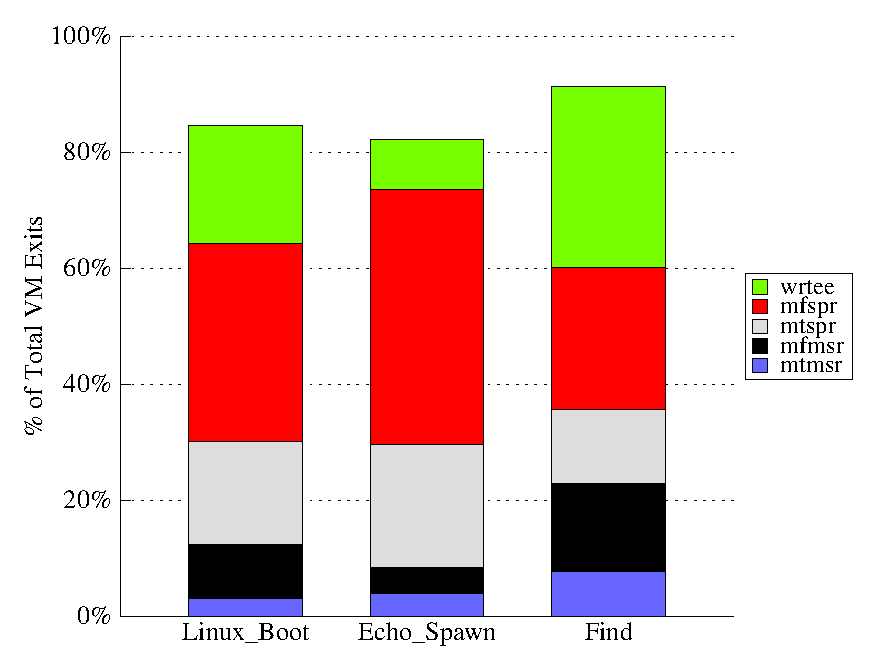
\includegraphics[scale=0.5]{exit_count.eps}
\caption{\label{fig:opcode_exit_fraction}Main sources of VM exits}
\end{figure}

\begin{table}[!b]
\centering
     \begin{tabular}{lcc} \hline
       Instruction class  & Exit count & \% of total exits  \\ \hline
       {\tt mfspr} & 4484245 & 33.8  \\
       {\tt wrtee} & 2792109 & 21.1  \\
       {\tt mtspr} & 2307647 & 17.4  \\
       {\tt mfmsr} & 575302 & 9.5 \\
       {\tt rfi} & 413847 & 4.3 \\
       {\tt mtmsr} & 391813 & 3.1 \\
       {\tt dtlbmiss} & 198239 & 1.5 \\
       {\tt itlbmiss} & 192046 & 1.4 \\
       \hline
     \end{tabular}
\caption{\label{tab:exitcount_linuxboot}Main sources of VM exits and their frequency on guest Linux boot (refer Table~\ref{tab:priv_opcodes} for semantics of these opcodes)}
\end{table}

\begin{table}
\centering
     \begin{tabular}{lcc} \hline
       Exits count  & PC count & \% of total exits  \\ \hline
       $>$20000 & 93 & 91.9  \\
       $>$10000 & 23 & 3.1  \\
       $>$5000 & 68 & 4.2  \\
       $>$2000 & 12 & 0.3 \\
       $>$1000 & 17 & 0.2 \\
       $<$1000 & 299 & 0.2 \\
       \hline
     \end{tabular}
\caption{\label{tab:pcexits_linuxboot}PCs responsible for VM exits on guest Linux boot}
\end{table}

\begin{figure}[!tb]
\centering
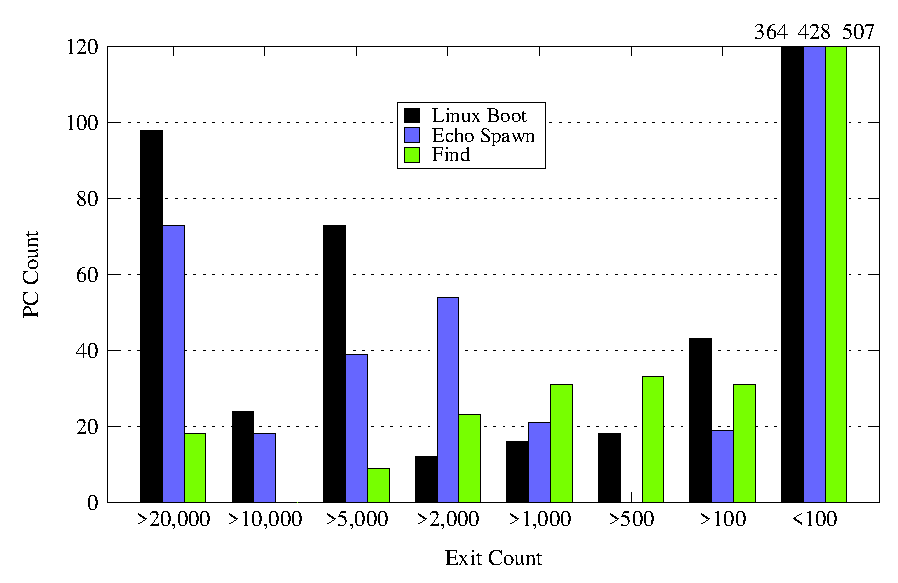
\includegraphics[scale=0.5]{pc_count.eps}
\caption{\label{fig:pc_profile}Exit Profile of Different Guest PCs for three different macrobenchmarks}
\end{figure}

Modifying the guest's address space has obvious pitfalls. Firstly, binary translation must ensure correctness in presence of arbitrary branches in the code. For example, it would be incorrect if the guest could potentially jump to the middle of the translated code. To ensure correctness, a privileged guest instruction is replaced by at most one translated instruction in the guest's address space. Because instructions are fixed length and word aligned on Power Architecture platform, this ensures that there can never be a branch to the middle of the translated code.

These translations to non-privileged VMM logic may be single line  or multi-line in nature. Some privileged opcodes can be emulated by single-instruction translations. For example, {\tt mfmsr} is translated to a {\tt load} instruction to the address of the emulated {\tt msr} register in the shared read/write page. Other opcodes which can be translated to single instructions are {\tt mfmsr}, {\tt mfspr} and {\tt mtspr}. These opcodes requiring single-instruction translations cause the bulk of privileged exits in common workloads (refer Figure~\ref {fig:opcode_exit_fraction}). We call the privileged instruction that was patched, the {\em patch-site}.

Other privileged opcodes require translation to multiple instructions. To implement multi-instruction translation, such instructions are instead replaced with a direct branch to a code fragment in a host-managed translation cache. This code fragment emulates the privileged instruction in guest's address space. The code fragment is terminated with another branch {\em back} to the instruction following the patch-site (see Figure~\ref{fig:txcache}). Because each patch-site requires a different terminating branch instruction, a new translation is generated for each patch-site. This branch is implemented as a single instruction in the guest's address space, and the translation cache is allocated in host's address space.

\begin{figure}[!tb]
\centering
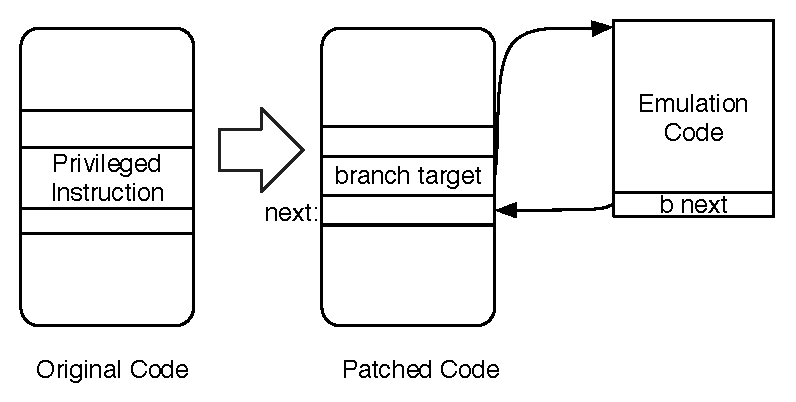
\includegraphics[scale=0.5]{txcache.eps}
\caption{\label{fig:txcache}Figure showing patching of multiple instructions with {\tt branch} instruction.}
\end{figure}

For the above scheme to work, the guest must have direct access to the translation cache in it's address space, but without it's knowledge.
We allocate the translation cache to an unused/unmapped region of the guest by inserting a (shadow) TLB entry in the guest's TLB. The physical memory for the translation cache is allocated on the host. The translation cache placement
has more constraints. Because a single Power Architecture direct branch
instruction can only specify a 26%XXX
bit signed offset
address the entire 32-bit address space, this places constraints on the placement of these data structures.

We now discuss the resulting placement constraints on these data structures. The translated code needs to access either the emulated guest state or the translation cache.  Single-instruction translations access the emulated state using load and store instructions. To avoid any register overwrites, these memory access instructions must encode the address within the opcode. Power Architecture ISA allows the specification of a signed 16-bit displacement. This implies that the emulated state must lie either in the top or bottom 32KB of the guest address space. If such address space is not available, single-instruction translations can be converted to multiple-instruction translations to allow more placement flexibility.

For multiple-instruction translations, the privileged instruction is replaced with a branch to the translation cache. Branch instructions are of two types: direct and indirect. An indirect branch would clobber the link register or will result in register overwrites. To prevent such clobbering patch multi-line instructions would have to be patched with multi-line translated code which poses the danger of a branch between the translated code as discussed earlier (see Figure~\ref{fig:multiple_insns_patching}). This limits the adaptive binary translator to use direct branches only. A direct branch in Power Architecture platform can only jump $\pm$32MB relative to it's location. This constrains the translation cache to lie within $\pm$32MB of the patch-site.

We found that it is not always possible to find unmapped guest virtual address space which satisfies these constraints. We present a scheme to steal guest’s address space and place these data structures in the stolen space.

\begin{figure}
\centering
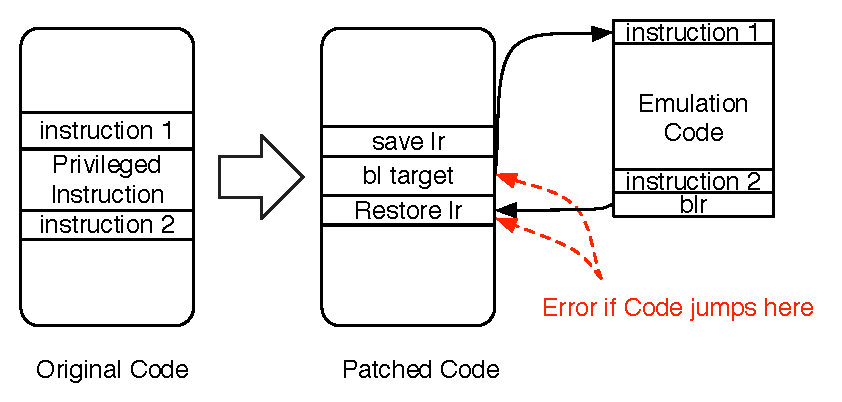
\includegraphics[scale=0.5]{multiple_ins_patching.eps}
\caption{\label{fig:multiple_insns_patching}Figure showing patching of multiple instructions using {\tt bl} instruction. This approach fails in presence of arbitrary guest jumps.}
\end{figure}

\section{Full Binary Translation}
\label{full_binary_translation}
We call a binary translator which translates all guest instructions a full binary translator. VMware’s x86-based binary translator\cite{adams:asplos06} is an example of such a system. A full binary translator translates all guest code. This can be done statically or dynamically. In static binary translation, the translator translates all the executable code statically to run on the target architecture. While dynamic binary translations translates a shorter sequence of code typically one basic block at a time on the fly during the guest's execution. It relies on the fact that only small portion of the code is executed majority of the times and thus caching the translations would reduce the overhead of doing the translations on the fly. Another major overhead during full binary translation is that translation of an indirect branch (e.g., function return) on a full binary translator incurs significant overhead due to a potential table lookup on each execution.

Full binary translation approach contrasts with the light-weight adaptive binary translation. While full binary translation translates all the guest code that is executed, light-weight adaptive binary translation only translates the privileged instructions. Since guest code is run natively with privileged instructions translated in case of light-weight adaptive binary translation it avoids both the overheads faced by the full binary translator. The disadvantage of light-weight adaptive binary translation is that it changes the guest address space directly and thus have to monitor the guest's accesses to the modified regions. As we demonstrate in this work, it is possible to do this correctly and efficiently using our proposed optimizations. The advantage of our approach is it’s simplicity and often higher performance.

Full Binary translation is a popular technique and has been previously used in various contexts, namely cross-ISA portability\cite{bansal:osdi08, qemu:software}, hardware-based performance acceleration\cite{transmeta_crusoe:chip}, runtime compiler optimizations\cite{bala00dynamo}, program shepherding \cite{bruening04thesis}, testing and debugging\cite{valgrind}. Binary translation was first used for efficient virtualization on the x86 architecture by VMware\cite{adams:asplos06}, and our work is perhaps closest to their approach. The difference is in the translator's design, as previously discussed.

\section{Memory Tracing}
\label{memory_tracing}
Memory tracing is a mechanism by which all the accesses to desired regions of memory by the guest can be tracked and emulated if necessary. It is used as a page-protection mechanism to protect a page from any read/write access by the guest. For e.g VMware’s x86-based binary translator\cite{adams:asplos06} uses {\tt memory tracing} to protect accesses (write) to in-memory privileged data such as page tables, memory mapped I/O devices. Tracing a page is done by removing the read/write prvileges form the hardware page protection bits to trap all accesses to the desired page. For example VMware’s x86-based binary translator uses tracing to prevent it's shadow page table entrys (PTEs) from becoming incoherent with the guest PTEs. It removes the read/write permissions from the memory containing the guest PTEs causing every access to guest PTEs get trapped. It then emulates its effect and reflects it in both the guest PTEs and shadow PTEs.



